\section{Ejercicio 3}

\subsection{Introducción}

El problema consiste en obtener la mínima suma posible de las longitudes de los pasillos que debemos clausurar para que no existan ciclos en el grafo y además sea conexo. 

\subsection{Desarrollo}
\label{des-ej3}

Lo que se nos pide sobre el grafo(debe ser conexo y no tener ciclos), es similar a buscar un árbol generador mínimo, con el detalle que tenemos que quedarnos con los pasillos
con mayor costo de cierre. Para lograr esto tenemos el algoritmo de Kruskal que, utilizando una estructura de Union-Find, podemos resolver correctamente este problema. 

\begin{comment}
Esta estructura utiliza dos diccionarios parametrizados con el tipo de los rótulos de los vértices, que almacenan rangos y padres de cada nodo, utilizados para las heurísticas de path-compression y union pesada. Estos diccionarios se implementan sobre la estructura TreeMap, que garantiza acceso e inserción con costo logarítmico.

La inicialización de la misma toma una lista de los elementos y les asigna a todos rango 0 y los pone como padre de si mismo. 
\end{comment}

Esta estructura utiliza dos arreglos donde se almacenan rangos y padres de cada nodo, utilizados para las heurísticas de path-compression y unión pesada.
Dado un tamaño del conjunto, se inicializan los arreglos colocando en cada posición a si misma como padre y 0 como rango.

Para obtener el representante del grupo de un elemento(\textit{find}) usamos el siguiente procedimiento:

\begin{itemize}
    \item Obtenemos el padre del elemento.
    \item Mientras el padre no sea igual a su padre(el único elemento de un conjunto que tiene como padre a si mismo es el representante) buscamos el siguiente padre.
    \item Asignamos al elemento al representante que encontramos en el anterior.
    \item Devolvemos el representante.
\end{itemize}

 Para unir dos conjuntos disjuntos(\textit{union}) realizamos los siguientes pasos:

\begin{itemize}
    \item Conseguimos los representantes de ambos conjuntos(usando \textit{find}).
    \item Si son iguales, ambos elementos pertenecen al mismo conjunto.
    \item Caso contrario:
    \begin{itemize}
         \item Conseguimos el rango de los dos y comparamos.
         \item Si el rango de uno es mayor que el de otro entonces el representante de ese pasa a ser el representante del representante del otro, en otras palabras ahora son un solo 
conjunto.
	 \item Si son iguales, desempatamos a favor del primero e incrementamos su rango.
    \end{itemize}
\end{itemize}

Gracias a la unión pesada y al path compression, estas operaciones tienen un costo cercano a $O(1)$.

Para resolver el problema, inicializamos primero las estructuras de soporte.
A partir de la lista de pasillos de entrada, construimos un \textit{max-heap} con todos sus elementos y obtenemos, a partir del máximo extremo nombrado en la lista de pasillos, la cantidad de esquinas. Adicionalmente, construimos una estructura union-find con tamaño igual a la cantidad de esquinas.

A partir de estas estructuras utilizamos el algoritmo de Kruskal con la particularidad de invertir el orden en que se recorren las aristas, dada por la utilización de un \textit{max-heap} en lugar de un \textit{min-heap}.

Implementamos este algoritmo de acuerdo al siguiente pseudocódigo:\\


\flushleft Estructuras que usamos:\\
\hspace{10pt}\textit{grafoUnionFind} Es una estructura Union-Find.\\
\hspace{10pt}\textit{colaDePasillos} Es un \textit{max-heap} donde tenemos a todos los pasillos de nuestro grafo.

\begin{algorithm}[H]
\caption{Desarmar Ciclos(Kruskal)}\label{init-ej3}
\begin{algorithmic}[6]
\Procedure{Inicialización}{Lista(Pasillos) pasillos}


\State $n \gets 0$		\Comment $O(1)$

\for{cada Pasillo \textit{pasillo} en \textit{pasillos}} 	\Comment $O(M Log M)$
  \State $n \gets \max\{n, \max\{pasillo.extremo1, pasillo.extremo2\}\}$ \Comment $O(1)$
  \State \textit{colaDePasillos.encolar(pasillo)}  \Comment $O(Log M)$
\EndFor
\State \textit{grafoUnionFind} $\gets$ \textit{CrearUnionFind(n)} \Comment $O(N)$ Con N la cantidad de esquinas

\EndProcedure
\end{algorithmic}
\end{algorithm}

\begin{algorithm}[H]
\caption{Desarmar Ciclos(Kruskal)}\label{alg-ej3}
\begin{algorithmic}[7]
\Procedure{Desarmar}{}
\State \textit{sumaPasillosEliminados} $\gets$ 0 		\Comment $O(1)$
\While{\textit{colaDePasillos} no vacía}     				
  \State \textit{pasillo} $\gets$ \textit{colaDePasillos.desencolar() }		\Comment $O(Log M)$
  \State \textit{e1 $\gets$ pasillo.extremo1}		\Comment $O(1)$
  \State \textit{e2 $\gets$ pasillo.extremo2}		\Comment $O(1)$
  
  
  \If{\textit{grafoUnionFind.conectado(e1, e2)}} 	\Comment $O(1)$		
    \State $sumaPasillosEliminados \gets sumaPasillosEliminados + pasillo.longitud$	\Comment $O(1)$
  \Else
    \State \textit{grafoUnionFind.union(e1, e2) }		\Comment $O(1)$ por path compression y union pesada
  \EndIf

\EndWhile

\Return \textit{sumaPasillosEliminados}
\EndProcedure
\end{algorithmic}
\end{algorithm}

Para cada pasillo, ordenado de mayor a menor por el \textit{max-heap}, controlamos si sus extremos están en el mismo conjunto Union-Find. Si es así, ese pasillo forma un ciclo y lo descartamos. En caso contrario unimos los dos extremos para representar que el pasillo forma parte del grafo final.

\subsection{Correctitud}

La demostración de correctitud de este algoritmo es análoga a la de Kruskal para árbol generador mínimo, pues solo difiere en que se analizan las aristas en orden inverso, de acuerdo a lo expuesto en el pseudocódigo \ref{alg-ej3}.
Utilizamos la demostración de la teórica cambiando los detalles necesarios para adecuarlo al árbol generador máximo.

Para ver que el algoritmo construye un árbol generador, como en cada paso el subgrafo B elegido hasta el momento es generador y acíclico, basta ver que el algoritmo termina
con $m_{B}$ = $n_{G}$ − 1. Si $m_{B}$ $<$ $n_{G}$ − 1, B es no conexo. Sea $B_{1}$ una componente conexa de B. Como G es conexo, va a existir alguna arista con un extremo en $B_{1}$ y el otro en V(G) − $B_{1}$, 
que por lo tanto no forma ciclo con las demás aristas de B. Entonces, si $m_{B}$ $<$ $n_{G}$ − 1, el algoritmo puede realizar un paso más.

Sea G un grafo, $T_{K}$ el árbol generado por el algoritmo de Kruskal y {$e_{1}$, $e_{2}$, . . . , $e_{n-1}$} la secuencia de aristas de $T_{K}$ en el orden en que fueron elegidas por el algoritmo 
de Kruskal. Para cada árbol generador T de G definimos l(T) como el máximo k $\leq$ n tal que $\forall$j $<$ k, $e_{j}$ $\not\in$ T.

Ahora, sea T un AGM que minimizar l(T). Si l(T) = n, entonces T coincide con $T_{K}$ , con lo cual $T_{K}$ resulta ser máximo. Si $T_{K}$ no es máximo, entonces l(T) $<$ n y $e_{l(T)}$ $\not\in$ T. 
Como T es conexo, en T hay un camino C que une los extremos de $e_{l(T)}$.

Como $T_{K}$ es acíclico, hay alguna arista e en C tal que e $\not\in$ $T_{K}$. Como $e_{1}$, . . . , $e_{l(T)−1}$ $\in$ T y T es acíclico, e no forma ciclos con $e_{1}$, . . . , $e_{l(T)−1}$. Por la forma en 
que fue elegida $e_{l(T)}$ por el algoritmo de Kruskal, peso($e_{l(T)}$) $\geq$ peso(e). Pero entonces $T_{0}$ = T − e $\cup$ {$e_{l(T)}$} es un árbol generador de G de peso mayor o igual a T y 
l($T_{0}$) $<$ l(T), absurdo.

Luego $T_{K}$ es un árbol generador máximo. 



\subsection{Complejidad}

La complejidad de consturir las estructuras es de $O(M log M)$, de acuerdo a lo expuesto en la sección \ref{des-ej3} y el pseudocódigo \ref{init-ej3}. Como el grafo original es conexo la cantidad de nodos es menor o igual a la cantidad de aristas mas 1. De esta manera, podemos acotar $O(N)$ con $O(M)$, y la complejidad de la inicialización queda dominada por la construcción del \textit{max-heap}.

Para la resolución usando Kruskal, de acuerdo a lo que señalamos en la sección de desarrollo (pseudocódigo \ref{alg-ej3}), consideremos que la complejidad de las operaciones de cada paso del ciclo se acota por $O(Log M)$, con M cantidad de aristas. Esto es lo que nos cuesta sacar el próximo elemento de la cola, la operación de mayor costo. Esto se repite para todas
las aristas, por lo tanto la complejidad de resolver por Kruskal es O(M Log M). Por último tenemos que la complejidad de armar la estructura y de resolver por Kruskal es, en peor caso, O(M Log M). Por lo tanto la complejidad con la que se resuelve el problema es de O(M Log M)



\subsection{Experimentación}

Se plantean una serie de casos de prueba para los cuales esperamos obtener resultados correctos en base a lo expuesto en las secciones anteriores.

Para empezar haremos un test usando un árbol que se forma por un camino lineal entre los nodos (del 1 al 4). Como lo que buscamos es el árbol generador entonces si el grafo
dado ya es un árbol entonces el resultado de aplicarle el algoritmo es 0 ya que no cerramos ningún camino.

%Tengo que hacer gráficos ilustrativos para todos estos experimentos.


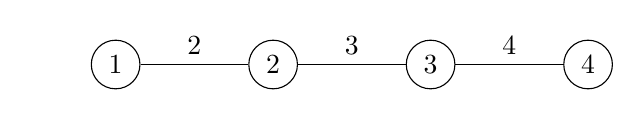
\begin{tikzpicture}
\node(pseudo) at (-1,0){};
\node(0) at (0,0)[shape=circle,draw]        {$1$};
\node(1) at (2,0)[shape=circle,draw]        {$2$};
\node(2) at (4,0)[shape=circle,draw]        {$3$};
\node(3) at (6,0)[shape=circle,draw] 	   {$4$};
\path [-]
  (0)      edge                 node [above]  {2}     (1)
  (1)      edge                 node [above]  {3}     (2)
  (2)      edge                 node [above]  {4}     (3);

\end{tikzpicture}

Para el segundo haremos lo mismo pero esta ves el árbol será un vértice unido a todas las demás aristas. Nuevamente el resultado es el mismo.

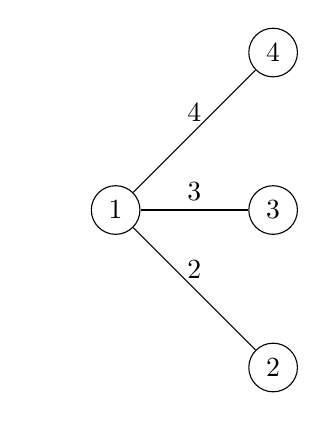
\begin{tikzpicture}
\node(pseudo) at (-1,0){};
\node(0) at (0,0)[shape=circle,draw]        {$1$};
\node(1) at (2,-2)[shape=circle,draw]        {$2$};
\node(2) at (2,0)[shape=circle,draw]        {$3$};
\node(3) at (2,2)[shape=circle,draw] 	   {$4$};
\path [-]
  (0)      edge                 node [above]  {2}     (1)
  (0)      edge                 node [above]  {3}     (2)
  (0)      edge                 node [above]  {4}     (3);

\end{tikzpicture}

En el tercero usaremos un grafo que sea un circuito simple con una arista menos pesada que las otras. Lógicamente se eliminarla esta sola y el resultado será el peso de la 
misma.

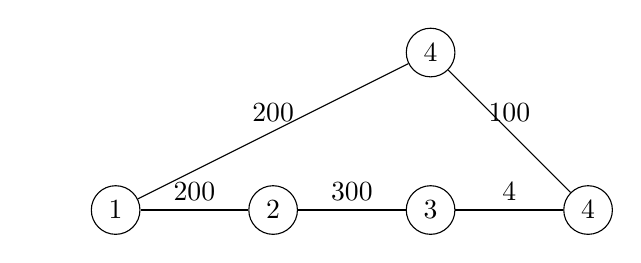
\begin{tikzpicture}
\node(pseudo) at (-1,0){};
\node(0) at (0,0)[shape=circle,draw]        {$1$};
\node(1) at (2,0)[shape=circle,draw]        {$2$};
\node(2) at (4,0)[shape=circle,draw]        {$3$};
\node(3) at (6,0)[shape=circle,draw] 	   {$4$};
\node(4) at (4,2)[shape=circle,draw] 	   {$4$};
\path [-]
  (0)      edge                 node [above]  {200}     (1)
  (1)      edge                 node [above]  {300}     (2)
  (2)      edge                 node [above]  {4}     (3)
  (0)      edge                 node [above]  {200}     (4)
  (4)      edge                 node [above]  {100}     (3);

\end{tikzpicture}

El siguiente es similar al anterior solo que usando una arista muy pesada y las otras poco pesadas. Nuevamente tenemos el mismo resultado, se elimina la menos pesada.

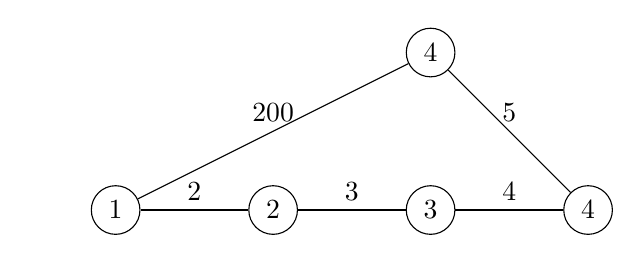
\begin{tikzpicture}
\node(pseudo) at (-1,0){};
\node(0) at (0,0)[shape=circle,draw]        {$1$};
\node(1) at (2,0)[shape=circle,draw]        {$2$};
\node(2) at (4,0)[shape=circle,draw]        {$3$};
\node(3) at (6,0)[shape=circle,draw] 	   {$4$};
\node(4) at (4,2)[shape=circle,draw] 	   {$4$};
\path [-]
  (0)      edge                 node [above]  {2}     (1)
  (1)      edge                 node [above]  {3}     (2)
  (2)      edge                 node [above]  {4}     (3)
  (0)      edge                 node [above]  {200}     (4)
  (4)      edge                 node [above]  {5}     (3);

\end{tikzpicture}


Por último tenemos un caso de circuitos múltiples. Variaremos los pesos de las aristas, dejando una mucho menos pesada que las otras.

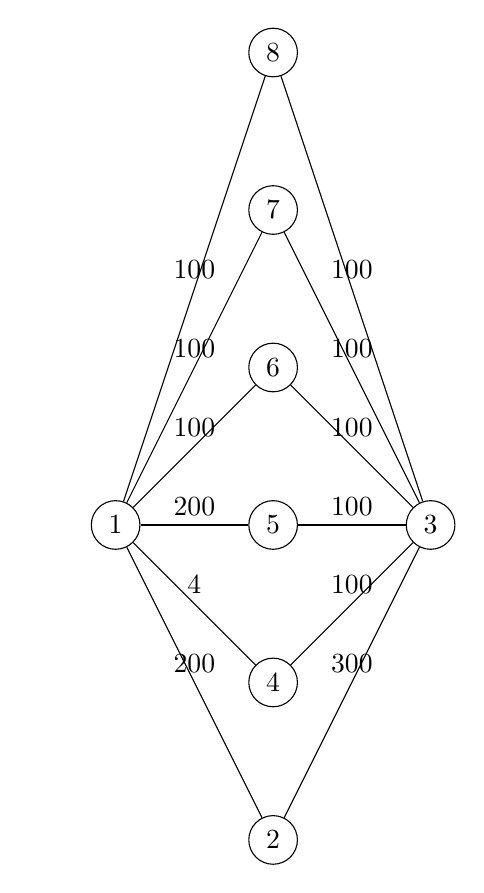
\begin{tikzpicture}
\node(pseudo) at (-1,0){};
\node(0) at (0,4)[shape=circle,draw]        {$1$};
\node(1) at (2,0)[shape=circle,draw]        {$2$};
\node(2) at (4,4)[shape=circle,draw]        {$3$};
\node(3) at (2,2)[shape=circle,draw] 	   {$4$};
\node(4) at (2,4)[shape=circle,draw] 	   {$5$};
\node(5) at (2,6)[shape=circle,draw]        {$6$};
\node(6) at (2,8)[shape=circle,draw] 	   {$7$};
\node(7) at (2,10)[shape=circle,draw] 	   {$8$};
\path [-]
  (0)      edge                 node [above]  {200}   (1)
  (0)      edge                 node [above]  {4}     (3)
  (0)      edge                 node [above]  {200}   (4)
  (0)      edge                 node [above]  {100}   (5)
  (0)      edge                 node [above]  {100}   (6)
  (0)      edge                 node [above]  {100}   (7)
  
  (1)      edge                 node [above]  {300}   (2)
  (3)      edge                 node [above]  {100}   (2)
  (4)      edge                 node [above]  {100}   (2)
  (5)      edge                 node [above]  {100}   (2)
  (6)      edge                 node [above]  {100}   (2)
  (7)      edge                 node [above]  {100}   (2);

\end{tikzpicture}

El resultado de este último es 404 que es lo que sale de haber cortado el pasillo de costo mínimo(4) y 4 pasillos de costo 100. Y con esto tenemos los distintos casos que Kruskal
resuelve correctamente, los demás grafos se conformaran de combinaciones de los anteriores entonces, si el algoritmo resuelve correctamente ejemplos similares a estos, 
podrá resolver los demás.
 

Para hacer las mediciones de tiempos generaremos los casos mejor y peor, luego tomaremos el tiempo de cada uno ejecutándolo 100 veces y tomando el promedio para 
garantizar que la medición es creíble. Variaremos la cantidad de vértices de los grafos generados así como las aristas que los unen. En estas mediciones obviamos el costo de preparar las estructuras, dado que tiene la misma complejidad temporal que el algoritmo que resuelve el problema.

El peor caso en nuestro algoritmo de Kruskal es cuando debemos conectar muchos de los vértices en el Union-Find. En otras palabras, no tenemos que quitar a nadie del grafo
para que este sea un árbol. La idea más obvia es usar un grafo que conecte linealmente los vértices, el primero con el segundo , el segundo con la tercero y así hasta
llegar al último. Los pesos de las aristas van variando entre más pesados y menos pesados para hacer más costoso el ordenamiento en la cola de prioridad. 
Para el mejor caso debemos considerar que, contrario a lo anterior, el mejor escenario es cuando tenemos que conectar pocas aristas respecto al total. La idea a la que se 
llego es un grafo completo, ya que debemos conectar n-1 aristas en comparación a las n-1*n/2 que tenemos para formar un árbol. Utilizamos todas las aristas con el mismo 
peso para no tener impacto en el orden.

\begin{figure}[H]
\input{plots/Tp2Ej3Exp1.tex}
\caption{Comparación de tiempos variando la cantidad de aristas, los valores del gráfico están escalados. El escalado es de 1:100}
\end{figure}

Para generar estas variaciones lo que hacemos es, en el mejor caso, tenemos un grafo completo lo que significa que para una cantidad de 100 vértices tendremos 4950 aristas.
Variamos la cantidad de vértices de 100 a 1000 con saltos de 100 para armar estos ejemplos. Para el peor caso tenemos un grafo en linea, por lo tanto tomamos las variaciones
del anterior y le aplicamos la función $i(i-1)/2$ para asegurarnos que los dos tienen la misma cantidad de aristas. 


